%!TEX root = /Users/ede/Documents/Master/19_AS/Ausarbeitung/as-ausarbeitung.tex
\section{Tag-Ranking Verfahren} % (fold)
\label{sec:tag_ranking_verfahren}
% TODO
Hier erfolgt die Darstellung der Tag-Ranking Verfahren im genauen. Und eine bessere Einleitung für dieses Kapitel.

TODO:

- bezug zw. {tag ranking, relevanz, ranking-wert, den beiden verfahren}, herstellen

- relevanz bezieht sich ja bei denen immer auf die schon vergebenen tags

% 
% 
% \begin{itemize}
%   \item   Visual diversification of image search results \cite{diversification}
%   \item   Tag ranking \cite{ranking}
%   \item   Learning to tag \cite{learningToTag}
%   \item   Learning tag relevance by neighbor voting for social image retrieval \cite{learningtagrelevance}
%   \item   Improving recommendation lists through topic diversification \cite{improvingRecommendations}
%   \item   Why we tag: motivations for annotation in mobile and online media \cite{whyWeTag}
%   \item   Flickr tag recommendation based on collective knowledge \cite{collectiveKnowledge}
% \end{itemize}

\subsection{Ranking basierend auf kollektivem Wissen nach Sigurbjörnsson und van Zwol} % (fold)
\label{sub:ranking_basierend_auf_kollektivem_wissen_nach_zwol}

Im Folgenden wird kurz das gesamte Verfahren von \cite{collectiveKnowledge} skizziert und anschließend näher erläutert. Das Verfahren produziert für vom Benutzer vergebene bzw. benutzerdefinierte Tags eine geordnete Liste von weiteren, zugehörigen Tags. Grundlage des Rankings ist die \emph{co-occurrence}, oder zu deutsch \emph{gemeinsames Auftreten}, von Tags bei unterschiedlichen Bildern. Diese Häufigkeitsgröße fließt zunächst in die Generierung einer Kandidatensequenz von zugehörigen Tags für jedes benutzerdefinierte Tag ein. Die Sequenz dient dann als Eingabe für die Tag Aggregation und das anschließende Tag Promotion, was die endgültige, nach Relevanz sortierte Liste von Tags ergibt. Abbildung \ref{fig:images_collective_knowledge_system_overview} veranschaulicht das System.

\begin{figure}[htbp]
  \centering
    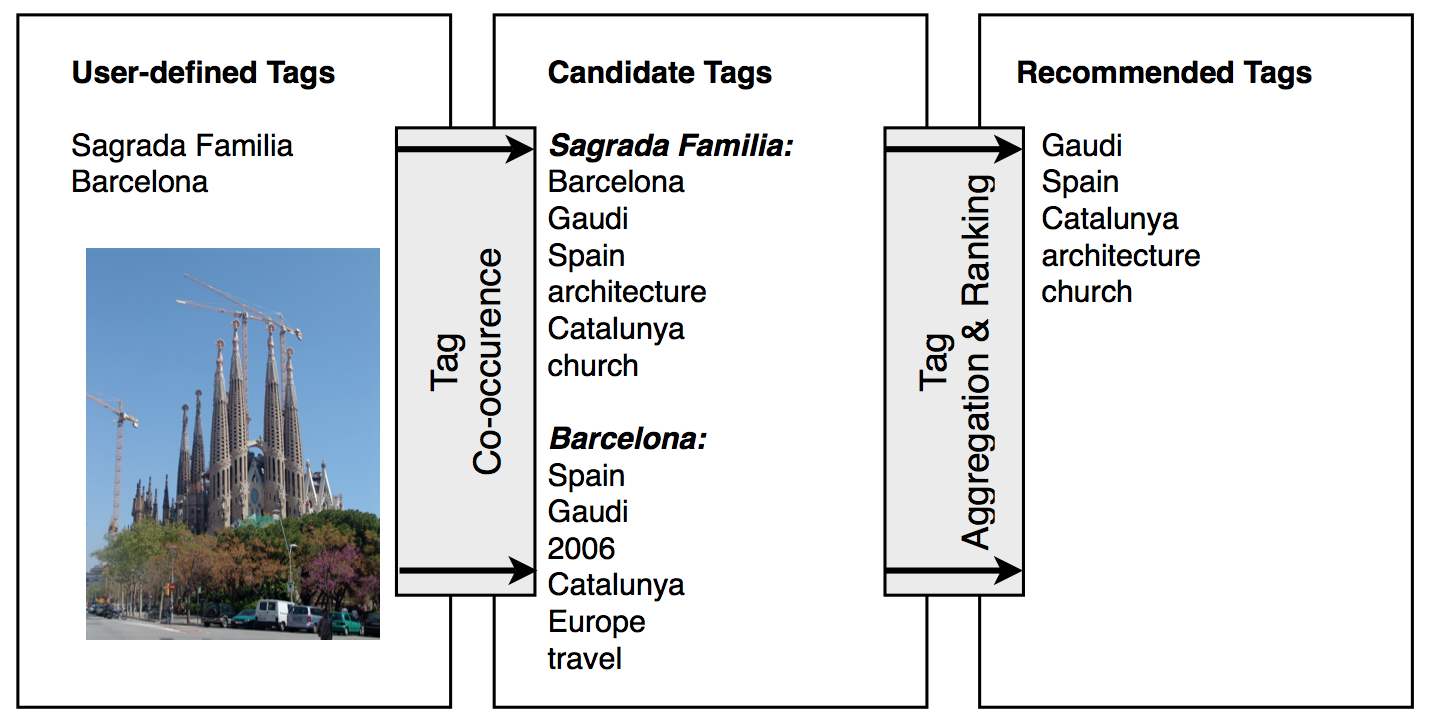
\includegraphics[height=3in]{images/collective_knowledge_system_overview.png}
  \caption{Übersicht des Tag Empfehlungssytems nach \cite{collectiveKnowledge}.}
  \label{fig:images_collective_knowledge_system_overview}
\end{figure}




% TODO:- Verfahren basiert auf Tag co-occurrence
% Tag co-occurrence is the key to our tag recommendation approach, and only works reliable when a large quantity of supporting data is available.

\subsubsection{Co-occurrence} % (fold)
\label{ssub:co_occurrence}

Die mathematische Definition von co-occurrence nach \cite{collectiveKnowledge} lautet \emph{``We define the co-occurrence between two tags to be the number of photos [in our collection] where both tags are used in the same annotation.''} 
 
 % - sehr einfache basis für verfahren
 
Um den Wert der co-occurrence von der allgemeinen Verwendungsfrequenz der Tags zu trennen wird dieser Wert normalisiert. Co-occurrence als Maßeinheit für das gemeinsame Auftreten von Tags kann auf unterschiedliche Weise normalisiert werden, was deutliche Auswirkung auf das Ergebnis hat.

Die symmetrischen Normalisierung gibt die Äquivalenz von zwei Tags, ${t_i}$ und ${t_j}$ an, da hierbei die Summe der Anzahl beider Tags als Divisor verwendet wird und somit die gemeinsame Auftrittswahrscheinlich für diese beiden Tags angegeben wird. Beispielsweise sind zu \emph{Eiffel Tower} als äquivalent gefundene Tags \emph{Tour Eiffel, Eiffel, Seine, La Tour Eiffel} und \emph{Paris}.
\begin{figure}[hptb]
  \begin{equation}
  \label{symmetricNormalization}
   J(t_i, t_j) := \frac{\vert t_i \cap t_j \vert}{ \vert t_i \cup t_j \vert }
  \end{equation}
\end{figure}

Die co-occurrence $J(t_i, t_j)$ ist also ein Koeffizient aus der Schnittmenge der Tags ${t_i}$ und ${t_j}$, und der Vereinigungsmenge von ${t_i}$ und ${t_j}$.

Bei der asymmetrischen Normalisierung wird die Anzahl des gemeinsamen Auftretens durch die Anzahl des ersten Tags dividiert. Damit wird also erfasst, wie oft ${t_i}$ gemeinsam mit ${t_j}$ gelistet wird, was beim Vorschlagen von Tags mehr Sinn macht, damit der Inhalt der Photos möglichst vielfältig anstatt genau getaggt werden kann. So ergibt der Tag \emph{Eiffel Tower} folgende Sequenz assoziierter Tags: \emph{Paris, France, Tour Eiffel, Eiffel} und \emph{Europe}.
% TODO: hier gibts kritikmöglichkeit, warum diese normaliesierung gewählt wurde, evtl. später aufgreifen.
\begin{figure}[hptb]
 \begin{equation}
 \label{asymmetricNormalization}
  P(t_i \vert t_j) := \frac{\vert t_i \cap t_j \vert}{ \vert t_i \vert }
 \end{equation}
\end{figure}

In Anbetracht der Aufgabe, die Medien möglichst vielfältig zu Taggen, wird die zweite Varianten von den Autoren verwendet.

Die normalisierten Werte für die co-occurrence fließen nun beim Vorschlagen von Tags in den Ranking Prozess ein. Zunächst wird für jeden vom Benutzer bereits vergebenen Tag $u$ eine Kandidatensequenz $C_u$ von Tags erstellt, wobei die Tags nach ihrem co-occurrence Wert zu dem jeweiligen benutzerdefinierten Tag geordnet sind.

Folgende unterschiedliche Typen von Tag Mengen werden in der Aggregation und dem Ranking verwendet:
\begin{itemize}
  \item Benutzerdefinierte Tags $U$ beziehen sich auf die zu einem Photo bereits vergebenen Tags.
  \item Kandidatentags $C_u$ bezeichnet die nach dem co-occurrence Wert geordnete Liste von $m$ Tags für einen Tag $u \in U$. Die Menge $C$ ist somit die Vereinigungsmenge aller Kandidatentags für jeden vom Benutzer vergebenen Tag $u$.
  \item Vorgeschlagene Tags $R$ ist die endgültige, vom System produzierte, geordnete Liste von $n$ höchst bewerteten Tags für ein Photo.
\end{itemize}

% subsubsection co_occurrence (end)


\subsubsection{Aggregation der Kandidatentags} % (fold)
\label{ssub:aggregation}

Bei der Aggregation werden die Kandidatensequenzen für die unterschiedlichen vom Benutzer vergebenen Tags zu einer einzigen geordneten Liste vereinigt. Dabei werden zwei unterschiedliche Strategien vorgeschlagen, deren Gemeinsamkeit darin besteht, dass sie jeweils über alle Kandidatentags iterieren. Die erste wertet Tags höher, die in mehreren Kandidatensequenzen vorkommen, die zweite betrachtet nur den Wert der co-occurrence für die Tags. 

Bei der \emph{voting strategy} werden die Tags $c \in C$ höher gewertet bzw. überhaupt gezählt, falls der Tag $c$ in der Menge $C_u$, also einer Kandidatensequenz, vorkommt. 
\begin{figure}[hptb]
 \begin{equation}
 \label{voteAggregation}
  vote(u, c)=\begin{cases}
    1, & \text{wenn } c \in C_u\\
    0, & \text{sonst }
  \end{cases}
 \end{equation}
\end{figure}

Der Ranking-Wert für einen Tag $c$ ergibt sich somit aus der Summe der \emph{votes}, wodurch sich auch die Sortierung der vorgeschlagenen Tags $R$ ergibt.

\begin{figure}[hptb]
 \begin{equation}
 \label{voteScoreAggregation}
    score(c) := \sum_{u \in U} vote(u, c)
 \end{equation}
\end{figure}


Die \emph{summing strategy} betrachtet hingegen den co-occurrence Wert zwischen den Tags $c$ und $u$. Für jeden Kandidatentag $c$ werden die asymmetrischen co-occurrence Werte zum Ranking-Wert $score(c)$ aufsummiert, falls dieser in der Kandidatensequenz $C_u$ für den benutzerdefinierten Tag $u$ enthalten ist. Das Ergebnis ist ebenfalls eine sortierte Menge von vorgeschlagenen Tags $R$.
\begin{figure}[hptb]
 \begin{equation}
 \label{sumScoreAggregation}
    score(c) := \sum_{u \in U} (P(c \vert u), \text{wenn } c \in C_u)
 \end{equation}
\end{figure}
% subsubsection aggregation (end)

Die unterschiedlichen Auswirkungen der beiden Ranking Strategien auf die Reihenfolge der vorgeschlagenen Tags $R$ werden im Kapitel \ref{sec:performance_und_skalierung} erläutert. 

\subsubsection{Promotion der Kandidatentags} % (fold)
\label{ssub:promotion}
Nach dem die Kandidatensequenzen $C_u$ für alle benutzerdefinierten Tags $u$ zu einer Sequenz von vorgeschlagenen Tags $R$ aggregiert wurden, erfolgt eine Auf- und Abwertung, von den Autoren \emph{promotion} genannt, der Ranking Werte der Tags.

Dabei fließen die Untersuchungsergebnisse aus Kapitel \ref{sec:analyse_und_klassifikation}, dass sehr oft benutzte Tags wenig aussagefähig sind sowie dass sehr selten benutzte Tags zu spezifisch sind, in diesen Schritt ein. Das als \emph{Stability-promotion} bezeichnete Ranking reduziert den Ranking Wert bei geringer Frequenz. Die \emph{Descriptiveness-promotion} wertet Tags mit sehr hoher Frequenz ab. So werden alle Tags in Relation zu ihrer Verwendungshäufigkeit nochmals bewertet. 

Beides sind Gewichtungsfunktionen (\ref{stabilityPromotion} und \ref{descriptivePromotion}) mit festen Parametern $k_s$ respektive $k_d$, die durch Training von den Autoren ermittelt wurden. $\vert u \vert$ bzw. $\vert c \vert$ ist die Verwendungshäufigkeit des Tags $u$ bzw. $c$ bezogen auf die gesamte Tag Menge. Die Funktion $abs(x)$ gibt den absoluten Wert von $x$ zurück.
\begin{figure}[hptb]
 \begin{equation}
 \label{stabilityPromotion}
    stability(u) := \frac{k_s}{k_s + abs(k_s - log(\vert u \vert))}
 \end{equation}
\end{figure}

\begin{figure}[hptb]
 \begin{equation}
 \label{descriptivePromotion}
    descriptive(c) := \frac{k_d}{k_d + abs(k_d - log(\vert c \vert))}
 \end{equation}
\end{figure}



Da der co-occurrence Wert sehr schnell abfällt, werden die Tags zusätzlich nach ihrer Reihenfolge in der Kandidatensequenz bewertet. Dies wird nach \cite{collectiveKnowledge} als \emph{Rank-promotion} bezeichnet. $r$ ist hierbei die Position des Tags $c \in C_u$ für einen benutzerdefinierten Tag $u$. Der Dämpfungsparameter $k_r$ wird ebenfalls durch Training ermittelt. 
\begin{figure}[hptb]
 \begin{equation}
 \label{rankPromotion}
    rank(u, c) = \frac{k_r}{k_r + (r-1)}
 \end{equation}
\end{figure}


Die kombinierte Gleichung für die Promotion ergibt sich aus einer Multiplikation der einzelnen Auf- und Abwertungen:
\begin{figure}[!hptb]
 \begin{equation}
 \label{combinedPromotion}
    promotion(u, c) := rank(u, c) \cdot stability(u) \cdot descriptive(c)
 \end{equation}
\end{figure}


Die zwei in Abschnitt \ref{ssub:aggregation} vorgestellten Methoden zur Aggregation werden jeweils mit und ohne Promotion von \cite{collectiveKnowledge} einzeln evaluiert. Eine mögliche Berechnung für den endgültigen Ranking Wert eines Kandidatentags mit der voting strategy und dem Einsatz vom Promotion ist in Gleichung \ref{finalRank} zu sehen.

\begin{figure}[!hptb]
 \begin{equation}
 \label{finalRank}
    score(c) :=  \sum_{u \in U} vote(u, c) \cdot promotion(u, c)
 \end{equation}
\end{figure}


Die Basis für das Training der Parameter $m,	k_r,	k_s, k_d$ wird in Kapitel \ref{sec:performance_und_skalierung} näher erläutert. 
% subsubsection promotion (end)

% subsection ranking_basierend_auf_kollektivem_wissen_nach_zwol (end)

\subsection{Verbesserung der Relevanz von Tags durch einen Random Walk nach Liu u. a.} % (fold)
\label{sub:verbesserung_der_relevanz_durch_einen_random_walk}

% - Initialwert ist zunächst für alle Tags gleich
% 
% - Zunächst Bestimmung des Wertes durch Beziehung zu Photos mit gleichen Tags, ähnliche dem Ansatz von \cite{collectiveKnowledge}. Dieser Wert ist die Gewichtung der Kanten zwischen zwei Tags/Knoten im folgenden Graph.
% 
% - Daraufhin wird ein Tag Graph erstellt, der als Basis für einen Random Walk dient. Vgl. \cite{} für Random Walk Literatur. 
% 
% - Dabei wird der Graph als Matrix mit den Ranking Werten formuliert. 
% 
% - Durch den Random Walk werden die Relevanzwerte durch die Gewichtung der Tags zu einander angepasst.
% Initialwert für den Rank eines Tags wird durch die Beziehung zwischen durch die Photos assoziierten Tags bestimmt. Für jedes Photo x mit den Nachbarn (haben den gleichen Tag) X

% Daraufhin erfolgt das Erstellen eines Tag Graphen

% \begin{itemize}
%   \item Wahrscheinlichkeitsorientierte Schätzung der Relevanz von Tags.
%   \item Random-Walk basierte Verfeinerung des Rankings
%     
%     \begin{itemize}
%       \item Aufbau eines Beziehungs-Graphen der Tags.
%       \item Random Walk über den Graphen
%     \end{itemize}
% \end{itemize}

% TODO: umformulieren, so dass das verfahren besser beschrieben wird.
Auch hier wird das Verfahren erst kurz in seiner Gesamtheit vorgestellt und anschließend im Detail betrachtet.
Das Tag Ranking Verfahren nach \cite{ranking} ist ebenfalls in 2 grundsätzliche Schritte aufgeteilt, hat jedoch einen anderen Ansatz zum Bewerten der Ranking Werte für einen Tag. So wird hierbei der Algorithmus nicht ausschließlich auf das Vorschlagen von Tags ausgerichtet. Weiterhin ist nicht allein die Beziehung zwischen zwei Tags von entscheidender Bedeutung, sondern alle Tags im System werden einem Ranking unterzogen und diese Ranking Werte fließen später in den Prozess der Vorschlagens ein. Weiterhin wirken sich die Ranking Werte von Tags auf verwandte Tags durch Einsatz von einem Random Walk aus. Abbildung \ref{fig:images_tag_ranking_verfahren} verdeutlicht schematisch den Ansatz.

\begin{figure}[htbp]
  \centering
    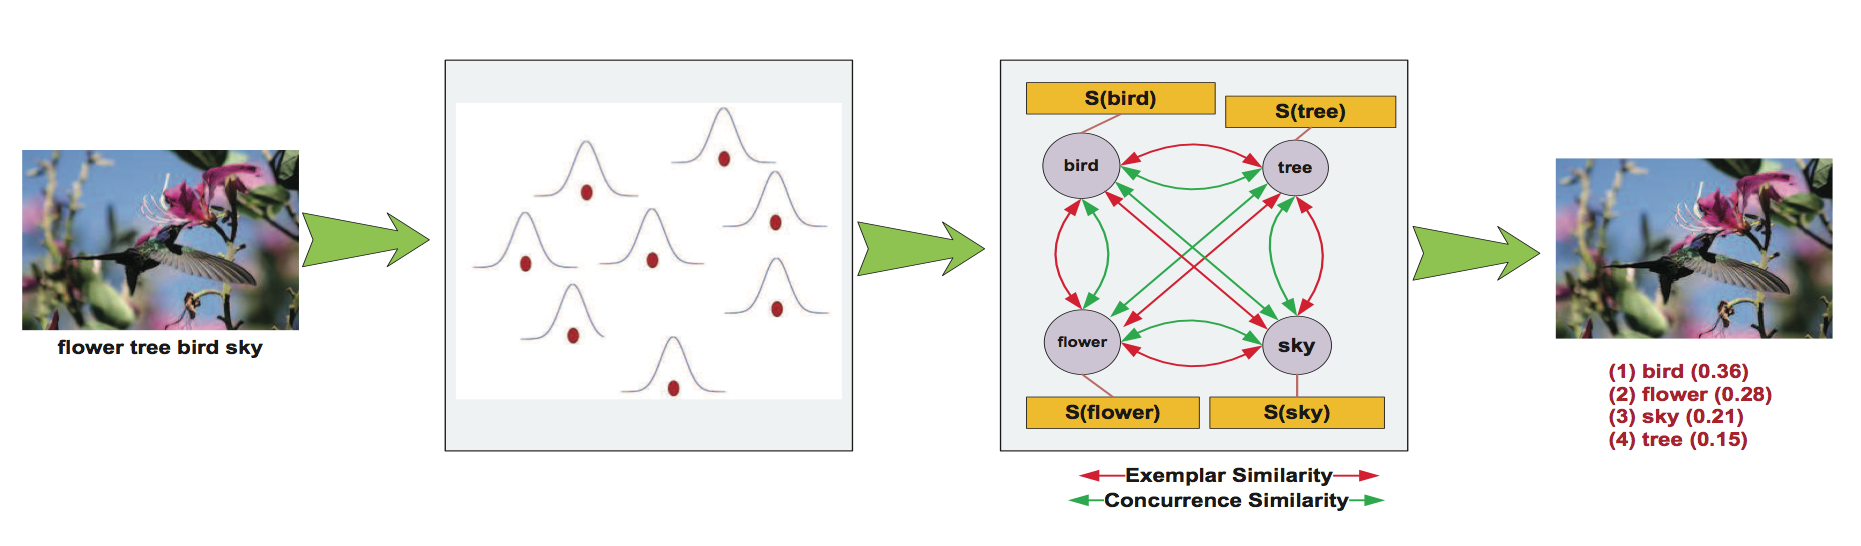
\includegraphics[height=1.8in]{images/tag_ranking_verfahren.png}
  \caption{Schema zum Tag Ranking Ansatz von \cite{ranking}.}
  \label{fig:images_tag_ranking_verfahren}
\end{figure}

Im ersten Schritt werden alle Photos durchlaufen und für alle zu einem Photo vergebenen Tags erfolgt eine Kerndichteschätzung. Hierbei fließen die Photos, die die gleichen Tags enthalten in die Berechnung mit ein. Dieser Schritt basiert also ebenfalls wie in der Methode von \cite{collectiveKnowledge} auf der co-occurrence von Tags. Im zweiten Schritt erfolgt der Aufbau eines Tag Graphen mit den Tags als Knoten und der Ähnlichkeit zwischen zwei Tags als Gewichtung der Kanten. Anschließend werden die Gewichte der Kanten durch einen Random Walk über den Graphen verfeinert, so dass die Relevanz einzelner Tags an ihre verbunden Tags weiter gereicht wird. Das Ergebnis des Verfahrens sind Relevanz bzw. Ranking Werte für alle Tags eines Photos.

Die Autoren von \cite{ranking} setzen den Ranking Wert gleich dem Relevanz Wert eines Tags. Somit hat ein Tag eine höhere Relevanz bezogen auf ein Bild je höher der Ranking Wert ist.

\subsubsection{Schätzung des Tag Relevanz Wertes} % (fold)
\label{ssub:schaetzung_des_tag_relevanz_wertes}

Im Unterschied zu \cite{collectiveKnowledge} wird hier über alle vorhandenen Bilder iteriert und für jeden Tag der Bilder ein Ranking Wert ermittelt. Hierbei wird der initiale Ranking Wert für ein Tag anhand eines Wahrscheinlichkeitstheoretischen Ansatzes, der Kerndichteschätzung, ermittelt.
 
% TODO: das raff ich nicht, aber hoffentlich raffts keiner, dass ich es nicht raff: was ist p(t)
 - Für einen Tag $t$ ist die Relevanz $s(t, x)$ zum Photo $x$ definiert als:
 \begin{figure}[hptb]
  \begin{equation}
  \label{fig:initialAsyncTagRelevance}
   s(t, x) = \frac{p(t \vert x)}{ p(t) }
  \end{equation}
 \end{figure}
 
Durch die in Gleichung \ref{fig:initialAsyncTagRelevance} vorgenommene Normalisierung der Wahrscheinlichkeit für das Auftreten von Tag $t$ beim Photo $x$ ausgedrückt durch $p(t \vert x)$, werden sehr häufig verwendete Tags abgewertet. Zum Beispiel liegt die Wahrscheinlichkeit für den Tag \emph{photo} bei jedem Photo bei 1, so dass durch seine häufige Frequenz nur wenig Aussagekraft hat. Durch Teilung mit der A-priori-Wahrscheinlichkeit, was in diesem Fall $p(t) = (1 / \text{Anzahl aller Tags})$ entspricht, wird der Relevanz Wert angepasst. Dieses Prinzip der Normalisierung ist im Gebiet des Information Retrieval breit erforscht und überprüft worden (vgl. \cite{bingLiu}) und wird heutzutage in vielen Gebieten eingesetzt, beispielsweise bei Googles PageRank Algorithmus aus \cite{googlePageRank}.
 
Nach dem Satz von Bayes\footnote{Der Satz von Bayes oder Bayestheorem sagt folgende Gesetzmäßigkeit für bedingte Wahrscheinlichkeiten aus: $P(A|B) = \frac{P(B \vert A) \cdot P(A)} {P(B)}$.\\ Hierbei ist $P(A)$ die A-priori-Wahrscheinlichkeit für ein Ereignis $A$ und $P(B \vert A)$ die Wahrscheinlichkeit für ein Ereignis $B$ unter der Bedingung, dass $A$ eingetreten ist und $P(B)$ die A-priori-Wahrscheinlichkeit für ein Ereignis $B$. } kann man die Formel vereinfachen zu:

\begin{figure}[hptb]
  \begin{equation}
  \label{fig:bayesInitialRelevance}
    s(t, x) = \frac{p(x \vert t)}{ p(t) }.
  \end{equation}
\end{figure} 

Da bei dem Algorithmus der Ranking Wert in Bezug zu einem Photo ermittelt wird und die Wahrscheinlichkeit $p(x)$ für ein Photo $x$ für alle zum Photo vergebenen Tags gleich ist, kann dieser Quotient entfernt werden, so dass $s(t,x) = p(x \vert t)$ gilt.

Um nun die explizite Wahrscheinlichkeitsfunktion aufzustellen, wird die Kerndichteschätzung, in englisch Kernel Density Estimation (KDE) genannt, adaptiert. Die Kerndichteschätzung oder auch Parzen-Methode nach \cite{parzen} ist ein Verfahren zur Darstellung einer eindimensionalen Verteilung. Diese Schätzung ist, im Gegensatz zu üblichen Darstellungsvarianten wie dem Histogramm, eine stetige Schätzung der unbekannten Verteilung. Die Verteilung bzw. die Stichprobe für ein zum Photo $x$ bereits vergebenen Tag $t_i$ ist hierbei die Menge der Photos $X_i$, in denen $t_i$ ebenfalls vorkommt. Damit berechnet die Kerndichteschätzung den Ranking Wert $s(t_i, x)$ folgendermaßen:

\begin{figure}[hptb]
  \begin{equation}
  \label{fig:kdeRelevance}
    s(t_i, x) = p(x \vert t_i) = \frac{1}{ \vert X_i \vert} \sum_{x_k \in X_i} K_{\sigma}(x - x_k)
  \end{equation}
\end{figure}

wobei $\vert X_i \vert$ die Kardinalität\footnote{Die Kardinalität oder Mächtigkeit einer endlichen Menge gibt die Anzahl ihrer Elemente an.} von $X_i$ ist und die Funktion $K_\sigma$ der Gaußkern der Kerndichteschätzung mit dem Radius Parameter $\sigma$ ist. Der Gaußkern ist in Gleichung \ref{fig:gaussKern} dargestellt.
\begin{figure}[hptb]
  \begin{equation}
  \label{fig:gaussKern}
    K_{\sigma}(x - x_k) = exp(-\frac{\vert \vert x - x_k \vert \vert^2}{ \sigma^2})
  \end{equation}
\end{figure}

Nach \cite{ranking} ist die Summe der \emph{Ähnlichkeiten} von Photos mit dem gleichen Tag, die mit der Gauß'schen Kernfunktion $K_\sigma$ berechnet wird, als Wertung der Photos $X_i$ für das Photo $x$ anzusehen. Der initiale Ranking Wert für einen Tag wird somit durch die Untersuchung von ``benachbarten'' Photos ermittelt. Je mehr Tags von den Photos geteilt werden, desto näher ist ihre Nachbarschaft.
% TODO: eigentlich beschreiben die autoren nicht was die euklidische distanz zwischen den Photos x udn x_k ist
% TODO: verstänldiche zusammenfassung, was nun das ergebnis der Kernfunktion ist.
% Je mehr Photos den gleichen Tag verwenden, desto höher ist sein Ranking Wert. 

% Das Ergebnis der Summe Schätzung für ein Tag $t_i$ eines Photos $x$ ist 


% subsubsection schaetzung_des_tag_relevanz_wertes (end)



\subsubsection{Konstruktion eines Tag Graphen} % (fold)
\label{ssub:konstruktion_eines_tag_graphen}

Der zweite Schritt des Verfahrens nach \cite{ranking} ist der aus dem Information Retrieval bekannte Random Walk, vgl. \cite{bingLiu}. Die Basis dafür ist ein gewichteter Graph. In diesem Fall repräsentieren die Knoten die Tags eines Photos und die Kanten zwischen den Tags werden mit zwei im folgenden beschriebenen Ähnlichkeitswerten gewichtet.
% TODO: auch hier wieder beschreiben die autoren nicht, wie sie zu der Menge der "repräsentativen photo Kollektion" kommen. in den Bilder steht etwas von Exemplarische Suche

Die \emph{exemplar similarity} bzw. exemplarische Ähnlichkeit $\varphi_e(t_i, t_j)$ beschreibt mit Hilfe der Gauß'schen Kernfunktion die Stärke der Ähnlichkeit zweier Tags $t_i$ und $t_j$. So sind die Tags \emph{cat}, \emph{animal} und \emph{kitten} stärker mit einander verbunden und haben damit auch einen höheren Ähnlichkeitswert zu einander als z.B. zum Tag \emph{Nikon}.

Die \emph{concurrence similarity} $\varphi_c(t_i, t_j) = exp(-d(t_i, t_j))$ bezieht sich auf das gemeinsame Auftreten von Tags bei Photos und wird analog zur Google Similarity Distance \cite{googleDistance} berechnet. Die Tag Ähnlichkeitsdistanz zwischen zwei Tags berechnet sich folgendermaßen:

\begin{figure}[hptb]
  \begin{equation}
  \label{fig:concurrenceDistance}
    d(t_i, t_j) = \frac{max(log f(t_i), log f(t_j)) - log f(t_i, t_j)}{log G - min(log f(t_i), log f(t_j))}
  \end{equation}
\end{figure}

Die Funktionen $f(t_i)$ und $f(t_j)$ geben die Anzahl der Photos an, in denen der Tag $t_i$ bzw. $t_j$ vorkommt, die Funktion $f(t_i, t_j)$ gibt die Anzahl der Photos in denen beide Tags vorkommen, an. $G$ ist die Anzahl aller Photos in Flickr.

Die Autoren legen die beiden Ähnlichkeitswerte zusammen und so ergibt sich die Gewichtung $s_{ij}$ der Kante zwischen den Tags $t_i$ und $t_j$:
\begin{figure}[hptb]
  \begin{equation}
  \label{fig:combinedSimilarity}
    s_{ij} = s(t_i, t_j) = \lambda \cdot \varphi_e(t_i, t_j) + (1 - \lambda) \cdot \varphi_c(t_i, t_j)
  \end{equation}
\end{figure}

wobei $\lambda$ der Menge $[0,1]$ entspricht und später festgelegt wird.

% subsubsection konstruktion_eines_tag_graphen (end)



\subsubsection{Random Walk über den Graphen} % (fold)
\label{ssub:random_walk_ueber_den_graphen}
Random Walk Verfahren sind im Information Retrieval etabliert und sollen hier nicht vertiefend dargestellt werden. Der Zweck des Verfahrens ist die Ausbreitung bzw. Weiterreichung der Ranking Werte über die Kanten des Graphen. Hat zum Beispiel der Tag \emph{cat} einen hohen Ranking Wert und ist dieser mit dem Tag \emph{animal} verbunden, so würde der Ranking Wert von \emph{cat} an \emph{animal} weiter gereicht werden. Dadurch wird erreicht, dass oft benutzte und damit verbundene Tags einen höheren Ranking Wert erhalten, da davon auszugehen ist, dass diese eine höhere Relevanz haben.

Der Random Walk ist ein iterativer Prozess und basiert auf homogenen Markoffschen Ketten, einem stochastischen Prozess \cite{bronstein}. Das Ergebnis des Random Walk für einen Graphen mit $n$ Knoten ist ein Spaltenvektor $\textbf{r}_k \equiv [r_k(i)]_{n \times 1}$. $r_k(i)$ ist hierbei der Ranking Wert des Knotens $i$ in der Iteration $k$. 

Um den Ranking Walk anzuwenden, wird der Graph in eine Matrixform gebracht. Matrix \textbf{P} ist somit eine $n \times n$ Transitions Matrix, wobei das Element $p_{ij}$ die Wahrscheinlichkeit für den Übergang von Knoten $i$ zum Knoten $j$ darstellt und wie folgt berechnet wird:
\begin{figure}[hptb]
  \begin{equation}
  \label{fig:probabilityScore}
    p_{ij} = \frac{s_{ij}}{\sum_k s_{ik}}.
  \end{equation}
\end{figure}

Damit kann nun der Random Walk Prozess für die Iteration $k$ folgendermaßen definiert werden:
\begin{figure}[hptb]
  \begin{equation}
  \label{fig:randomWalk}
    r_k(j) = \alpha \sum_i r_{k-1}(i)p_{ij} + (1 - \alpha)v_j.
  \end{equation}
\end{figure}

$v_j$ ist der initial geschätzte Wert für den Tag $t_j$ und $\alpha$ ist ein Gewichtungsparamter zwischen 0 und 1. Der Prozess konvergiert aufgrund der Eigenschaften von Markoffschen Ketten in einer endlichen Anzahl an Iterationen zu einem Vektor $r_\pi$. Der Beweis hierfür wird in dieser Ausarbeitung nicht angeführt.


% subsubsection random_walk_ueber_den_graphen (end)
\begin{figure}[htbp]
  \centering
    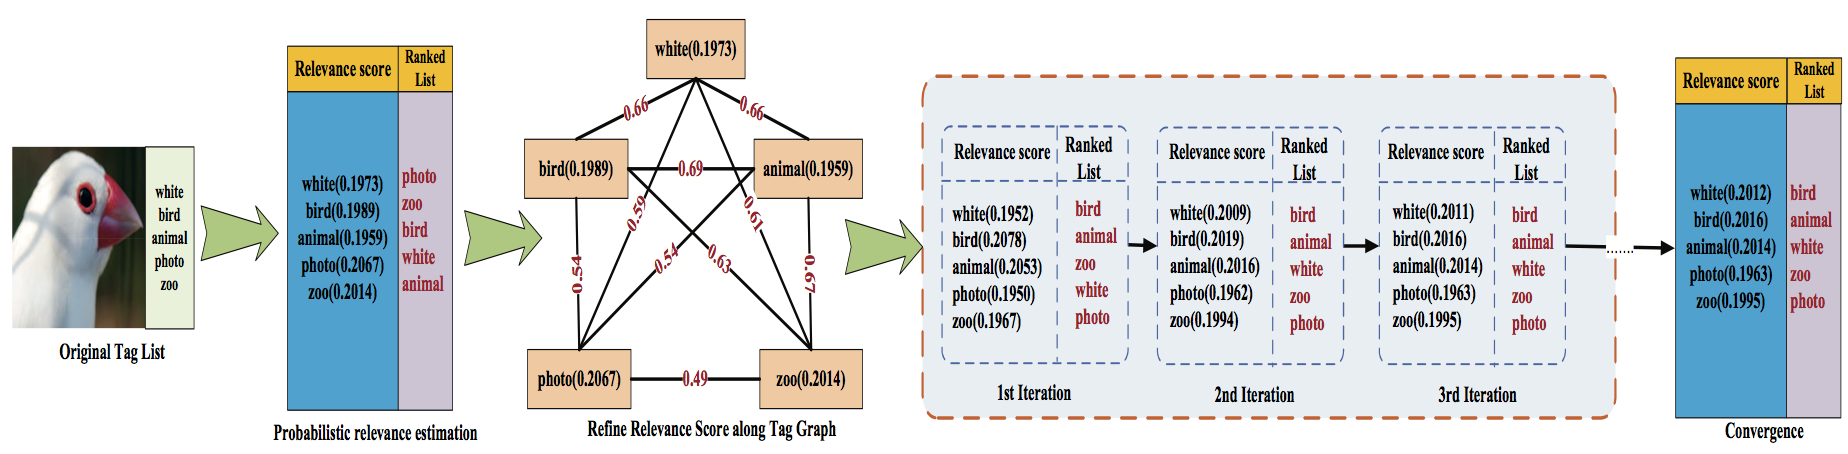
\includegraphics[height=1.5in]{images/example_of_random_walk.png}
  \caption{Beispiel für den gesamten Ranking Prozess nach \cite{ranking}.}
  \label{fig:randomWalkExample}
\end{figure}


Das Ergebnis des gesamten Prozesses ist ein Ranking von Tags eines Photos. In Abbildung \ref{fig:randomWalkExample} ist der Prozess am Beispiel eines Bildes illustriert. % Mittel Bildung von Durchschnitten über alle Photos und Tags hinweg können nun auch absolute Werte




% subsection verbesserung_der_relevanz_durch_einen_random_walk (end)

% section tag_ranking_verfahren (end)
